\section{Auswertung}
\label{sec:Auswertung}  

\subsection{Überprüfung der Aussagekraft der Messwerte}
\label{sec:Überprüfung}
Die Messwerte für die Spannungen von $\SI{150}{\volt}$, $\SI{170}{\volt}$, $\SI{190}{\volt}$, $\SI{210}{\volt}$
und $\SI{240}{\volt}$ sind \autoref{tab:t12}, \autoref{tab:t34} und \autoref{tab:t5} zu finden. Die gemessenen  
Thermistorwiderstände sind im Bereich von $\SI{1,895}{\mega\ohm}$ bis $\SI{1,922}{\mega\ohm}$, so dass nach der
im Anhang angegeben \autoref{fig:thermistor} für Thermistorwiderstände die
Temperatur zu $T\approx \SI{27}{\celsius} = \SI{301,5}{\kelvin}$ ablesbar ist. Es wurden nur Tröpfchen untersucht,
die keine Geschwindigkeit ohne angelegtes E-Feld haben, so dass die Messung von $t_{\symup{0}}$ nicht notwendig
ist. Die einzige Bewegung die die Tröpfchen aufgewiesen haben lässt sich durch die Brownsche Molekülbewegung
erklären und ist für $v_{\symup{0}}$ nicht von Relevanz, so dass sich für alle Tröpfchen
$v_{\symup{0}} = \SI{0}{\milli\meter\per\second}$ ergibt.
\begin{table}
  \centering
  \caption{Messwerte für $U=\SI{150}{\volt}$ und
  $U=\SI{170}{\volt}$.}
  \label{tab:t12}
  \begin{tabular}{c c c}
    \toprule
    Tröpfchen & $t_{\symup{ab}}/\unit{\second}$ & $t_{\symup{auf}}/\unit{\second}$ \\
    \midrule
    1 & 5,50 & 6,84 \\
      & 5,89 & 7,35 \\
      & 5,54 & 5,70 \\
    2 & 3,89 & 3,71 \\
      & 3,13 & 3,87 \\
      & 3,86 & 5,21 \\
    3 & 2,32 & 2,72 \\
      & 2,99 & 1,81 \\
      & 2,35 & 2,91 \\
    4 & 3,72 & 4,98 \\
      & 4,40 & 5,16 \\
      & 4,14 & 5,14 \\
    5 & 5,68 & 6,26 \\
      & 5,58 & 5,96 \\
      & 5,37 & 5,72 \\
    \bottomrule
  \end{tabular}
  \quad
  \begin{tabular}{c c c}
    \toprule
    Tröpfchen & $t_{\symup{ab}}/\unit{\second}$ & $t_{\symup{auf}}/\unit{\second}$ \\
    \midrule
    1 & 3,05 &  3,70 \\
      & 3,66 &  3,63 \\
      & 3,40 &  3,55 \\
    2 & 3,02 &  2,42 \\
      & 2,41 &  3,32 \\
      & 2,31 &  2,71 \\
    3 & 3,59 & 10,57 \\
      & 4,14 & 11,45 \\
      & 4,28 & 10,04 \\
    4 & 3,80 &  5,90 \\
      & 3,81 &  5,95 \\
      & 3,62 &  5,76 \\
    5 & 4,15 &  4,90 \\
      & 4,34 &  4,83 \\
      & 4,21 &  4,79 \\
    \bottomrule
  \end{tabular}
\end{table}

\begin{table}
  \centering
  \caption{Messwerte für $U=\SI{190}{\volt}$ und
  $U=\SI{210}{\volt}$.}
  \label{tab:t34}
  \begin{tabular}{c c c}
    \toprule
    Tröpfchen & $t_{\symup{ab}}/\unit{\second}$ & $t_{\symup{auf}}/\unit{\second}$ \\
    \midrule
    1 & 2,37 &  1,52 \\
      & 1,97 &  2,02 \\
      & 1,95 &  2,13 \\
    2 & 2,19 &  2,67 \\
      & 2,25 &  2,44 \\
      & 2,31 &  1,64 \\
    3 & 4,53 &  4,44 \\
      & 4,53 &  4,88 \\
      & 3,81 &  4,53 \\
    4 & 2,87 &  2,76 \\
      & 2,67 &  2,99 \\
      & 2,47 &  2,61 \\
    5 & 9,11 & 12,91 \\
      & 6,39 &  7,30  \\
      & 5,07 &  6,50  \\
    \bottomrule
  \end{tabular}
  \quad
  \begin{tabular}{c c c}
    \toprule
    Tröpfchen & $t_{\symup{ab}}/\unit{\second}$ & $t_{\symup{auf}}/\unit{\second}$ \\
    \midrule
    1 & 3,30 & 3,41 \\
      & 2,80 & 3,28 \\
      & 3,36 & 3,48 \\
    2 & 2,04 & 2,37 \\
      & 2,25 & 2,25 \\
      & 2,19 & 2,03 \\
    3 & 3,66 & 5,19 \\
      & 3,53 & 5,09 \\
      & 3,50 & 4,81 \\
    4 & 4,80 & 3,34 \\
      & 3,64 & 3,63 \\
      & 3,72 & 3,88 \\
    5 & 2,13 & 1,03 \\
      & 1,31 & 1,56 \\
      & 1,60 & 1,81 \\
    \bottomrule
  \end{tabular}
\end{table}

\begin{table}
  \centering
  \caption{Messwerte für $U=\SI{240}{\volt}$.}
  \label{tab:t5}
  \begin{tabular}{c c c}
    \toprule
    Tröpfchen & $t_{\symup{ab}}/\unit{\second}$ & $t_{\symup{auf}}/\unit{\second}$ \\
    \midrule
    1 & 1,75 & 1,95 \\
      & 2,24 & 2,14 \\
      & 2,35 & 2,51 \\
    2 & 2,33 & 6,03 \\
      & 3,66 & 5,51 \\
      & 3,19 & 6,22 \\
    3 & 1,78 & 1,25 \\
      & 1,35 & 1,57 \\
      & 1,88 & 1,61 \\
    4 & 1,79 & 2,19 \\
      & 1,79 & 1,95 \\
      & 2,19 & 2,40 \\
    5 & 2,24 & 2,75 \\
      & 2,36 & 2,79 \\
      & 2,46 & 2,77 \\
    \bottomrule
  \end{tabular}
\end{table}
Die Tröpfchen haben bei den gemessenen Zeiten einen Abstand von $s=\SI{0,5}{\milli\meter} = \SI{0,05}{\centi\meter}$
zurückgelegt, so dass sich aus den $t_{\symup{ab}}$ und $t_{\symup{auf}}$ die Geschwindigkeiten $v_{\symup{ab}}$ und
$v_{\symup{auf}}$ bestimmen lassen. Um sicher zu stellen, dass die Ladung sich während der Messung nicht
geändert hat, wird überprüft, ob
\begin{align*}
  2v_{\symup{0}} \approx v_{\symup{ab}} - v_{\symup{auf}}
\end{align*}
gilt. Mit $v_{\symup{0}}$ ergibt sich
\begin{align*}
  0 \approx v_{\symup{ab}} - v_{\symup{auf}}
\end{align*}
Die ermittelten Werte sind in \autoref{tab:Geschwindigkeit} zu finden. Insgesamt lässt sich fest stellen, dass
für die meisten Geschwindigkeitsdifferenzen der Tröpfchen in einem Intervall, das Null mit einschließt, liegen.
Die Geschwindigkeitsdifferenzen der Tröpfchen, für die das nicht gilt, sind so nah dran, dass trotzdem die
Bedingung gilt. Lediglich die Werte bei denen die Geschwindigkeitsdifferenz negativ ist werden nicht verwendet,
da mit ihnen keine Auswertung möglich ist.
\begin{table}
  \centering
  \caption{Geschwindigkeiten der Tröpfchen.}
  \label{tab:Geschwindigkeit}
  \begin{tabular}{c | c c c}
    \toprule
    Tröpfchen & $v_{\symup{ab}}/10^{-5}\frac{\si{\meter}}{\si{\second}}$ & $v_{\symup{auf}}/10^{-5}\frac{\si{\meter}}{\si{\second}}$ &
    $\left(v_{\symup{ab}} - v_{\symup{auf}}\right)/10^{-5}\frac{\si{\meter}}{\si{\second}}$ \\
    \midrule
    $  1 $ & $  8,86 \pm 0,28 $ & $  7,50 \pm 8,00 $ & $ 1,30 \pm 0,80 $ \\
    $  2 $ & $ 13,80 \pm 1,30 $ & $ 11,70 \pm 1,90 $ & $ 2,10 \pm 2,30 $ \\
    $  3 $ & $ 19,60 \pm 2,40 $ & $ 20,00 \pm 4,00 $ & $-1,00 \pm 5,00 $ \\
    $  4 $ & $ 12,20 \pm 0,80 $ & $ 09,82 \pm 0,16 $ & $ 2,40 \pm 0,90 $ \\
    $  5 $ & $ 09,02 \pm 0,21 $ & $ 08,36 \pm 0,31 $ & $ 0,70 \pm 0,40 $ \\
    $  6 $ & $ 14,80 \pm 1,10 $ & $ 13,79 \pm 0,23 $ & $ 1,10 \pm 1,10 $  \\
    $  7 $ & $ 19,40 \pm 2,40 $ & $ 17,80 \pm 2,40 $ & $ 1,60 \pm 3,30 $  \\
    $  8 $ & $ 12,50 \pm 0,90 $ & $ 04,68 \pm 0,25 $ & $ 7,80 \pm 1,00 $  \\
    $  9 $ & $ 13,36 \pm 0,31 $ & $ 08,52 \pm 0,12 $ & $ 4,84 \pm 0,33 $  \\
    $ 10 $ & $ 11,81 \pm 0,22 $ & $ 10,33 \pm 0,10 $ & $ 1,48 \pm 0,24 $  \\
    $ 11 $ & $ 23,80 \pm 2,20 $ & $ 26,00 \pm 4,00 $ & $-3,00 \pm 4,00 $ \\
    $ 12 $ & $ 22,20 \pm 0,50 $ & $ 22,00 \pm 4,00 $ & $ 0,00 \pm 4,00 $ \\
    $ 13 $ & $ 11,70 \pm 0,90 $ & $ 10,80 \pm 0,40 $ & $ 0,80 \pm 1,00 $ \\
    $ 14 $ & $ 18,70 \pm 1,10 $ & $ 17,90 \pm 1,00 $ & $ 0,80 \pm 1,50 $ \\
    $ 15 $ & $ 07,30 \pm 1,80 $ & $ 05,60 \pm 1,80 $ & $ 1,70 \pm 2,50 $ \\
    $ 16 $ & $ 15,90 \pm 1,30 $ & $ 14,70 \pm 0,40 $ & $ 1,10 \pm 1,30 $ \\
    $ 17 $ & $ 23,10 \pm 0,90 $ & $ 22,60 \pm 1,40 $ & $ 0,60 \pm 1,70 $ \\
    $ 18 $ & $ 14,03 \pm 0,27 $ & $ 09,94 \pm 0,32 $ & $ 4,10 \pm 0,40 $ \\
    $ 19 $ & $ 12,30 \pm 1,60 $ & $ 13,80 \pm 0,80 $ & $-1,50 \pm 1,80 $ \\
    $ 20 $ & $ 30,00 \pm 6,00 $ & $ 34,00 \pm 8,00 $ & $-4,00 \pm 10,00 $ \\
    $ 21 $ & $ 23,70 \pm 2,90 $ & $ 22,70 \pm 2,40 $ & $ 1,00 \pm 10,00 $ \\
    $ 22 $ & $ 16,30 \pm 2,90 $ & $ 08,40 \pm 0,40 $ & $ 7,90 \pm  4,00 $ \\
    $ 23 $ & $ 30,00 \pm 4,00 $ & $ 34,00 \pm 4,00 $ & $-4,00 \pm  3,00 $ \\
    $ 24 $ & $ 26,00 \pm 2,50 $ & $ 22,90 \pm 1,90 $ & $ 3,10 \pm  6,00 $ \\
    $ 25 $ & $ 21,20 \pm 0,80 $ & $ 18,05 \pm 0,11 $ & $ 3,20 \pm  0,80 $ \\
    \bottomrule
  \end{tabular}
\end{table}

\subsection{Bestimmung der Ladung und des Radius der Öltröpfchen}
\label{sec:LadRad}
Aus \autoref{eqn:q} und \autoref{eqn:r} lassen sich nun die Ladungen und der Radius der Tröpfchen bestimmen.
Die Viskosität der Luft lässt sich aus der im Anhang angegebenen \autoref{fig:viskositaet} zu $\eta_{\symup{L}}
=1,8575\cdot 10^{-5}\si{\newton\second\per\meter^2}$ ablesen. Die Dichte der Luft beträgt $\rho_{\symup{L}}=
\SI{1,204}{\kg\per\meter^3}$ und die für Öl beträgt $\rho_{\symup{Öl}}=\SI{886}{\kg\per\meter^3}$. Die Viskosität
wird in \autoref{eqn:r} und \autoref{eqn:q} durch die Korrektur nach Cunningham in \autoref{eqn:Korrekturterm}
bestimmt. Die elektrische Feldstärke des Plattenkondensators lässt sich aus dem Zusammenhang
$E=\frac{U}{d}$ mit $d=(7,6250 \pm 0,0051)\,\si{\milli\meter}$ bestimmen. Die korrigierte Ladung
ergibt sich aus \autoref{eqn:qKorr}. Die ermittelten Werte sind in \autoref{tab:q}
abgebildet.

\begin{table}
  \centering
  \caption{Radien, Ladungen und korrigierte Ladungen der Tröpfchen.}
  \label{tab:q}
  \begin{tabular}{c | c c c c}
    \toprule
    Tröpfchen & $U/\si{\volt}$ & $r/10^{-7}\si{\meter}$ & $q/10^{-19}\si{\coulomb}$ & $q_{\symup{korr}}/10^{-19}\si{\coulomb}$ \\
    \midrule
     1 & $150$ & $3,60 \pm 1,10$  & $1,3 \pm 0,4$   & $1,77 \pm 0,34$   \\
     2 & $150$ & $4,50 \pm 2,50$  & $2,5 \pm 1,3$   & $3,20 \pm 1,30$   \\
     3 & $150$ & $-$              & $-$             & $-$               \\
     4 & $150$ & $4,80 \pm 0,90$  & $2,4 \pm 0,5$   & $3,00 \pm 0,50$   \\
     5 & $150$ & $2,50 \pm 0,70$  & $9,7 \pm 2,7$   & $1,48 \pm 0,26$   \\
     6 & $170$ & $3,20 \pm 1,70$  & $1,8 \pm 1,0$   & $2,50 \pm 1,00$   \\
     7 & $170$ & $4,00 \pm 4,00$  & $2,9 \pm 3,0$   & $3,80 \pm 2,90$   \\
     8 & $170$ & $8,70 \pm 0,50$  & $2,92 \pm 0,33$ & $3,34 \pm 0,35$   \\
     9 & $170$ & $6,83 \pm 0,23$  & $2,93 \pm 0,14$ & $3,47 \pm 0,14$   \\
    10 & $170$ & $3,78 \pm 0,31$  & $1,64 \pm 0,15$ & $2,20 \pm 0,15$   \\
    11 & $190$ & $-$              & $-$             & $-$               \\
    12 & $190$ & $-$              & $-$             & $-$               \\
    13 & $190$ & $2,80 \pm 1,70$  & $1,1 \pm 0,7$   & $1,60 \pm 0,70$   \\
    14 & $190$ & $2,70 \pm 2,70$  & $1,8 \pm 1,7$   & $2,60 \pm 1,70$   \\
    15 & $190$ & $4,00 \pm 3,00$  & $0,9 \pm 0,7$   & $1,20 \pm 0,70$   \\
    16 & $210$ & $3,30 \pm 1,90$  & $1,6 \pm 1,0$   & $2,20 \pm 1,00$   \\
    17 & $210$ & $2,40 \pm 3,50$  & $1,7 \pm 2,5$   & $2,70 \pm 2,40$   \\
    18 & $210$ & $6,28 \pm 0,32$  & $2,39 \pm 0,12$ & $2,87 \pm 0,12$   \\
    19 & $210$ & $-$              & $-$             & $-$               \\
    20 & $210$ & $-$              & $-$             & $-$               \\
    21 & $240$ & $3,00 \pm 6,00$  & $2,0 \pm 4,0$   & $3,00 \pm 4,00$   \\
    22 & $240$ & $8,70 \pm 1,60$  & $3,0 \pm 0,9$   & $3,40 \pm 1,00$   \\
    23 & $240$ & $-$              & $-$             & $-$               \\
    24 & $240$ & $5,40 \pm 2,80$  & $3,7 \pm 2,0$   & $4,60 \pm 2,00$   \\
    25 & $240$ & $5,50 \pm 0,70$  & $3,0 \pm 0,4$   & $3,70 \pm 0,50$   \\
    \bottomrule
  \end{tabular}
\end{table}

\subsection{Bestimmung der Elementarladung}
\label{sec:Elementarladung}
Die korrigierten Ladungen sind in \autoref{fig:plot1} dargestellt. Die Elementarladung ist dabei der größte
gemeinsame Teiler der Ladungen. Die Nummerierung der Messungen wird wie in \autoref{tab:Geschwindigkeit}
beibehalten, so dass nach 5 Messwerten die Spannung erhöht wird und eine neue Messreihe begonnen wird. Um den
größten gemeinsamen Teiler zu bestimmen, wird nun der minimale Abstand der bestimmten Ladungen einer Messreihe,
der größer als $1\cdot 10^{-19}\,\si{\coulomb}$ ist, da der größte gemeinsame Teiler für fehlerbehaftet nicht
ganzzahlige Größen nicht bestimmbar ist. Anschließend werden die ermittelten Werte für $e_{\symup{0}}$
und $e_{\symup{0, korr.}}$ gemittelt.
\begin{figure}
  \centering
  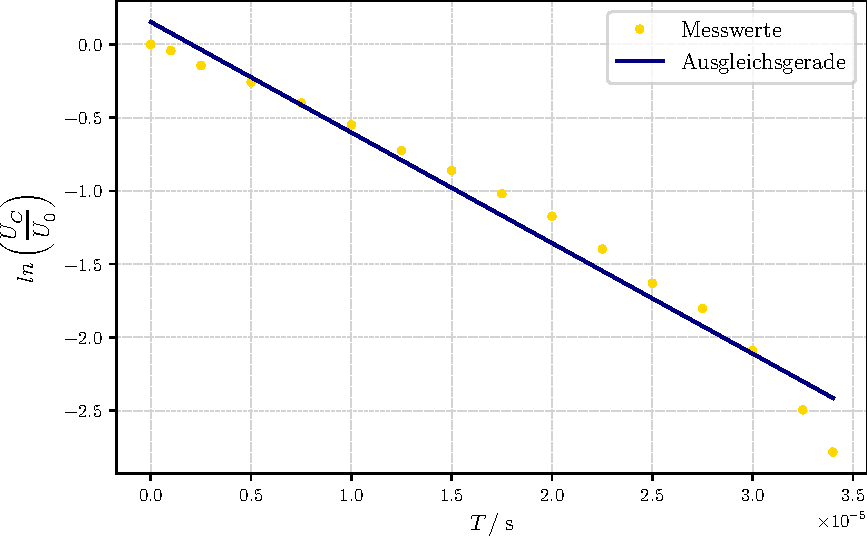
\includegraphics{plot1.pdf}
  \caption{Korrigierte Ladungen.}
  \label{fig:plot1}
\end{figure}
Die bestimmten Elementarladungen für die Ladung und die korrigierte Ladung sind in \autoref{tab:e} abgebildet.
Für die vierte Messreihe lässt sich dabei weder ein $e_{\symup{0}}$ noch ein $e_{\symup{0, korr}}$ bestimmen
und für die dritte Messreihe lässt sich kein $e_{\symup{0}}$ bestimmen.
\begin{table}
  \centering
  \caption{Elementarladungen mit und ohne Korrektur nach Cunningham und deren Mittelwerte.}
  \label{tab:e}
  \begin{tabular}{c c c c}
    \toprule
    Messreihe & $U/\si{\volt}$ & $e_{\symup{0}}/10^{-19}\si{\coulomb}$ & $e_{\symup{0, korr}}/10^{-19}
    \si{\coulomb}$ \\
    \midrule
    1           & $150$ & $1,1 \pm 0,6$ & $1,2 \pm 0,6$ \\
    2           & $170$ & $1,1 \pm 1,1$ & $1,1 \pm 0,4$ \\
    3           & $190$ &               & $1,0 \pm 1,8$ \\
    4           & $210$ &               &               \\
    5           & $240$ & $1 \pm 4$     & $2,0 \pm 4,0$ \\
    Mittelwert  &       & $1,1 \pm 1,4$ & $1,3 \pm 1,2$ \\
    \bottomrule
  \end{tabular}
\end{table}

\subsection{Berechnung der Avogadro-Konstante}
\label{sec:Avogadro}
Die Avogadrokonstane ist durch
\begin{align*}
  N_{\symup{A}} = \frac{F}{e_{\symup{0}}}
\end{align*}
definiert. Dabei ist die $F$ die Faradykonstante und beträgt $F= (96.485,3399 \pm 0,0024)\,\frac{\si{\coulomb}}
{\si{\mol}}$ \cite{faraday}. Mit $e_{\symup{0, korr}}$ eingesetzt ergibt sich
\begin{align*}
  N_{\symup{A}} = (8 \pm 7)\cdot 10^{23} \, \frac{1}{\si{\mol}}.
\end{align*}